\begin{longtable}{|S{c}|S{c}|S{c}|}
  % 1. DEFINIMOS EL PIE DE LA TABLA (AQUÍ VA EL CAPTION PARA QUE SALGA ABAJO)
  \hline
   \caption{Ejemplos de grafos con coloraciones}
  \addtocounter{table}{-1}\refstepcounter{table}% <-- Notifica a cleveref que es una tabla
  \label{tab:coloraciones_grafos} \\
  \endlastfoot
  
  % =========================================================
  % 2. A PARTIR DE AQUÍ VA EL CUERPO DE LA TABLA
  % =========================================================
  \hline
  % FILA 1: Nombres de los grafos
  \textbf{$G_1$} & \textbf{$G_2$} & \textbf{$G_3$} \\
  \hline
  
  % FILA 2: Grafos centrados en sus casillas
  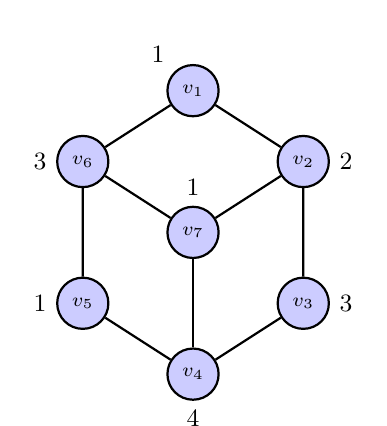
\begin{tikzpicture}[
  baseline=0pt,
  scale=1,
  vnode/.style={circle, draw=black, fill=blue!20, thick, inner sep=0pt, minimum size=6.5mm},
  edge/.style={thick, draw=black},
  clabel/.style={font=\small, color=black}
]
  \useasboundingbox (-2.1,-2.3) rectangle (2.1,2.4);

  \begin{scope}[yshift=-0.2cm]
    % 7 Vértices
    \node[vnode, label={[clabel]above left:$1$}] (v1) at (0.0, 1.8) {$\scriptstyle v_1$};
    \node[vnode, label={[clabel]right:$2$}]        (v2) at (1.4, 0.9) {$\scriptstyle v_2$};
    \node[vnode, label={[clabel]right:$3$}]        (v3) at (1.4, -0.9) {$\scriptstyle v_3$};
    \node[vnode, label={[clabel]below:$4$}]        (v4) at (0.0, -1.8) {$\scriptstyle v_4$};
    \node[vnode, label={[clabel]left:$1$}]         (v5) at (-1.4, -0.9) {$\scriptstyle v_5$};
    \node[vnode, label={[clabel]left:$3$}]         (v6) at (-1.4, 0.9) {$\scriptstyle v_6$};
    \node[vnode, label={[clabel]above:$1$}]        (v7) at (0.0, 0.0) {$\scriptstyle v_7$};

    % Aristas
    \draw[edge] (v1) -- (v2) -- (v3) -- (v4) -- (v5) -- (v6) -- (v1);
    \draw[edge] (v7) -- (v2);
    \draw[edge] (v7) -- (v6);
    \draw[edge] (v7) -- (v4);
  \end{scope}
\end{tikzpicture}
 &
  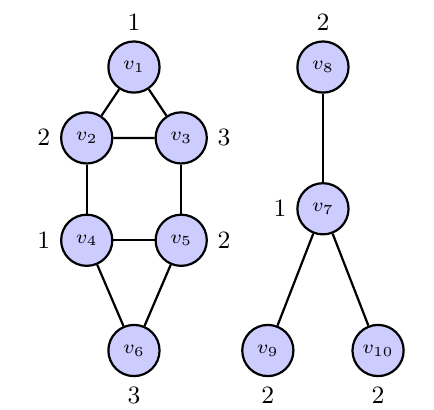
\begin{tikzpicture}[
  baseline=0pt,
  scale=1,
  vnode/.style={circle, draw=black, fill=blue!20, thick, inner sep=0pt, minimum size=6.5mm},
  edge/.style={thick, draw=black},
  clabel/.style={font=\small, color=black}
]
  % Se amplía xmin a -2.55 para añadir el medio carácter de margen izquierdo
  \useasboundingbox (-2.55,-2.2) rectangle (2.25,2.3);

  % --- COMPONENTE 1 ---
  \node[vnode, label={[clabel]above:$1$}] (v1) at (-1.2, 1.8) {$\scriptstyle v_1$};
  \node[vnode, label={[clabel]left:$2$}]  (v2) at (-1.8, 0.9) {$\scriptstyle v_2$};
  \node[vnode, label={[clabel]right:$3$}] (v3) at (-0.6, 0.9) {$\scriptstyle v_3$};
  \node[vnode, label={[clabel]left:$1$}]  (v4) at (-1.8, -0.4) {$\scriptstyle v_4$};
  \node[vnode, label={[clabel]right:$2$}] (v5) at (-0.6, -0.4) {$\scriptstyle v_5$};
  \node[vnode, label={[clabel]below:$3$}] (v6) at (-1.2, -1.8) {$\scriptstyle v_6$};

  \draw[edge] (v1) -- (v2) -- (v3) -- (v1);
  \draw[edge] (v2) -- (v4);
  \draw[edge] (v3) -- (v5);
  \draw[edge] (v4) -- (v5);
  \draw[edge] (v4) -- (v6);
  \draw[edge] (v5) -- (v6);

  % --- COMPONENTE 2 ---
  \node[vnode, label={[clabel]left:$1$}]  (v7)  at (1.2, 0.0) {$\scriptstyle v_7$};
  \node[vnode, label={[clabel]above:$2$}] (v8)  at (1.2, 1.8) {$\scriptstyle v_8$};
  \node[vnode, label={[clabel]below:$2$}] (v9)  at (0.5, -1.8) {$\scriptstyle v_9$};
  \node[vnode, label={[clabel]below:$2$}] (v10) at (1.9, -1.8) {$\scriptstyle v_{10}$};

  \draw[edge] (v7) -- (v8);
  \draw[edge] (v7) -- (v9);
  \draw[edge] (v7) -- (v10);
\end{tikzpicture}
 &
  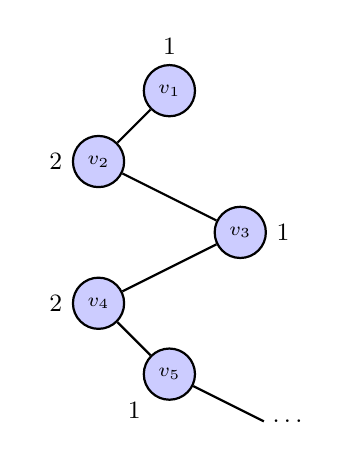
\begin{tikzpicture}[
  baseline=0pt,
  scale=1,
  vnode/.style={circle, draw=black, fill=blue!20, thick, inner sep=0pt, minimum size=6.5mm},
  edge/.style={thick, draw=black},
  clabel/.style={font=\small, color=black}
]
  % Caja delimitadora simétrica (-1.8 a 1.8) para centrar el eje x = 0
  \useasboundingbox (-1.8,-2.8) rectangle (1.8,2.4);

  \begin{scope}[yshift=-0.2cm]
    % Primeros 5 vértices
    \node[vnode, label={[clabel]above:$1$}]        (v1) at (0.0, 1.8) {$\scriptstyle v_1$};
    \node[vnode, label={[clabel]left:$2$}]         (v2) at (-0.9, 0.9) {$\scriptstyle v_2$};
    \node[vnode, label={[clabel]right:$1$}]        (v3) at (0.9, 0.0) {$\scriptstyle v_3$};
    \node[vnode, label={[clabel]left:$2$}]         (v4) at (-0.9, -0.9) {$\scriptstyle v_4$};
    \node[vnode, label={[clabel]below left:$1$}] (v5) at (0.0, -1.8) {$\scriptstyle v_5$};

    % Aristas
    \draw[edge] (v1) -- (v2) -- (v3) -- (v4) -- (v5);
    \draw[edge] (v5) -- (1.2, -2.4);
    \node[font=\small] at (1.5, -2.4) {$\dots$};
  \end{scope}
\end{tikzpicture}
 \\
  \hline
  
  % FILA 3: Funciones alineadas
  $\begin{aligned}[t]
      c_1 \!:\phantom{o} V(G_1) &\to \{1, 2, 3, 4\} \\
     v_1 &\mapsto 1 \\
     v_2 &\mapsto 2 \\
     v_3 &\mapsto 3 \\
     v_4 &\mapsto 4 \\
     v_5 &\mapsto 1 \\
     v_6 &\mapsto 3 \\
     v_7 &\mapsto 1
  \end{aligned}$ 
  &
  $\begin{aligned}[t]
     c_2 \!:\phantom{o} V(G_2) &\to \{1, 2, 3\} \\
     v_1 &\mapsto 1 \\
     v_2 &\mapsto 2 \\
     v_3 &\mapsto 3 \\
     v_4 &\mapsto 1 \\
     v_5 &\mapsto 2 \\
     v_6 &\mapsto 3 \\
     v_7 &\mapsto 1 \\
     v_8 &\mapsto 2 \\
     v_9 &\mapsto 2 \\
     v_{10} &\mapsto 2
  \end{aligned}$ 
  &
  $\begin{aligned}[t]
     c_3 \!:\phantom{o} V(G_3) &\to \{1, 2\} \\
     v_i &\mapsto 
     \begin{cases} 
       1 & \begin{array}[t]{@{}l@{}} \text{si } i \text{ es} \\[-1ex] \text{impar} \end{array} \\[0.6ex]
       2 & \begin{array}[t]{@{}l@{}} \text{si } i \text{ es} \\[-1ex] \text{par} \end{array} 
     \end{cases}
  \end{aligned}$ \\
  \hline
\end{longtable}
